\documentclass[a4paper,14pt]{extarticle} % the default article class is limited to 12pt, but you can go up to 14, 17 or 20 points if you use the extarticle class:
\usepackage{cmap} % make LaTeX PDF output copy-and-pasteable
\usepackage[T2A]{fontenc}
\usepackage[utf8]{inputenc}
\usepackage[english,ukrainian]{babel}

\usepackage{amssymb,amsfonts,mathtools,amsmath,cite,enumerate,float}
\usepackage{indentfirst} % set an additional space before a paragraph at the begining of new section
\usepackage{setspace}
\usepackage{textcomp}

\usepackage{import} % for adding a file by path https://tex.stackexchange.com/questions/246/when-should-i-use-input-vs-include

\usepackage{geometry} 
\geometry{left=1.25cm}
\geometry{right=1.25cm}
\geometry{top=1cm}
\geometry{bottom=2cm}

\usepackage[table,xcdraw,dvipsnames]{xcolor}
\usepackage{color}
% 1) tutorial about xcolor:  https://www.overleaf.com/learn/latex/Using_colours_in_LaTeX
% 2) huge tutorial about xcolor: https://latex-tutorial.com/color-latex/ 
% 3) RGB calculator: https://www.w3schools.com/colors/colors_rgb.asp

\usepackage{hyperref}
\definecolor{linkcolor}{HTML}{0000FF}
\definecolor{urlcolor}{HTML}{0000FF} 
\hypersetup{pdfstartview=FitH, linkcolor=linkcolor, urlcolor=urlcolor, colorlinks=true}

\usepackage{graphicx}
\usepackage{wrapfig}
\graphicspath{{Screenshots/}} % path to images

\parskip=1mm %space between paragraphs

\usepackage{listingsutf8} % for code (origin: \usepackage{listings})

\lstset{
    frame=single, %lines
    language=Python,
    aboveskip=3mm,
    belowskip=3mm,
    columns=flexible,
    basicstyle={\small\ttfamily},
    numbers=left,
    numberstyle=\tiny\color{gray},
    commentstyle=\color{OliveGreen},
    stringstyle=\color{Mahogany},
    morestring=[b]''',
    showstringspaces=false,
    keywordstyle=\bfseries\color{blue},
    emph={[1]import, as, for, return}, emphstyle={[1]\bfseries\color{magenta}},
    emph={[2]range}, emphstyle={[2]\bfseries\color{brown}},
    breaklines=true,
    breakatwhitespace=true,
    tabsize=4,
    extendedchars=false, % to use ukrainian text in a code
    inputencoding=utf8 % to use ukrainian text in a code
}

\begin{document}

\import{Title/}{title}

\newpage

\section*{Мета}

Ознайомитись з основами керування ресурсами AWS засобами Python SDK.

\section*{Завдання} 

\begin{itemize}
    \item Розробити Python-скрипт для автоматичного створення та видалення хмарної інфраструктури з 
    мінімальною конфігурацією (необхідно передбачити у функціях додаткові виключення для коректної роботи у 
    нестандартних ситуаціях (наприклад, виводити відповідне повідомлення при створення бакету з вже існуючим 
    ім’ям, при читанні з S3 файлу, якого там немає);
    \item Для результатів Лабораторної роботи \textnumero2 розробити bash-скрипт, який склонує код з 
    попередньо створеного git-репозиторію та встановить потрібні заленості \texttt{pip}.
\end{itemize}

\section*{Хід виконання роботи}

\subsection*{1. Автоматизація роботи з обчислювальними ресурсами EC}

\subsubsection*{Підготовчий етап}

Повторимо усі кроки Лабораторної роботи \textnumero1 стосовно встановлення інстансу й роботи з ним, проте тепер 
не через інтерфейс AWS, а засобами Python SDK. Перш за все маємо виконати деякі підготовчі кроки на власному 
локальному середовищі (тобто на ноутбуці чи комп'ютері):
\begin{enumerate}
    \item \textbf{Встановити мову Python3:} для операційної системи Ubuntu 20.04 (попередньо оновивши дерево пакетів) 
    це можна зробити за допомогою команди 
    \begin{align*}
        &\texttt{sudo apt update} \\
        &\texttt{sudo apt install python3}
    \end{align*}
    Для керування програмними пакетами мови Python3 наступним кроком слід встановити інструмент \texttt{pip}: 
    \[ \texttt{sudo apt install python3-pip} \]

    \item \textbf{Встановити бібліотеку Boto3:} для цього виконуємо одну просту команду 
    \[ \texttt{pip3 install boto3} \]
    Результат пункту зображений на Рис. \ref{fig:EC2:downloading boto3}.

    \item \textbf{Мати обліковий запис на AWS:} акаунт на AWS був створений ще у Лабораторній роботі \textnumero1. 
    Зараз постає завдання підключитися до цього акаунту з локального середовища. Скористаємося інструментами 
    AWS Command Line Interface (AWS CLI). Встановимо власне засоби AWS CLI командою
    \[ \texttt{sudo apt install awscli} \]
    Одразу хочу зауважити, що при некоректній роботі щойно встановлених інструментів (та і просто для профілактики, 
    як показав досвід другої лабораторної роботи, здійснимо превентивне виправлення несправностей, так би мовити) 
    виконаємо рядок
    \[ \texttt{pip3 install {-}{-}upgrade awscli} \]

    Усі проміжні результати на цей момент показані на Рис.~\ref{fig:EC2:downloading awscli}.

    Ну і наостанок власне здійснимо саме підключення до користувача AWS. Як це було виконано у Лабораторній 
    роботі \textnumero2, виконуємо команду 
    \[ \texttt{aws configure} \]
    й коректно заповнюємо усі параметри, скориставшись 
    \href{https://docs.aws.amazon.com/cli/latest/userguide/cli-configure-files.html}{інструкцією}. На 
    Рис.~\ref{fig:EC2:connecting to aws} можемо бачити успішне підключення до AWS.
\end{enumerate}

\begin{figure}[H]
    \center{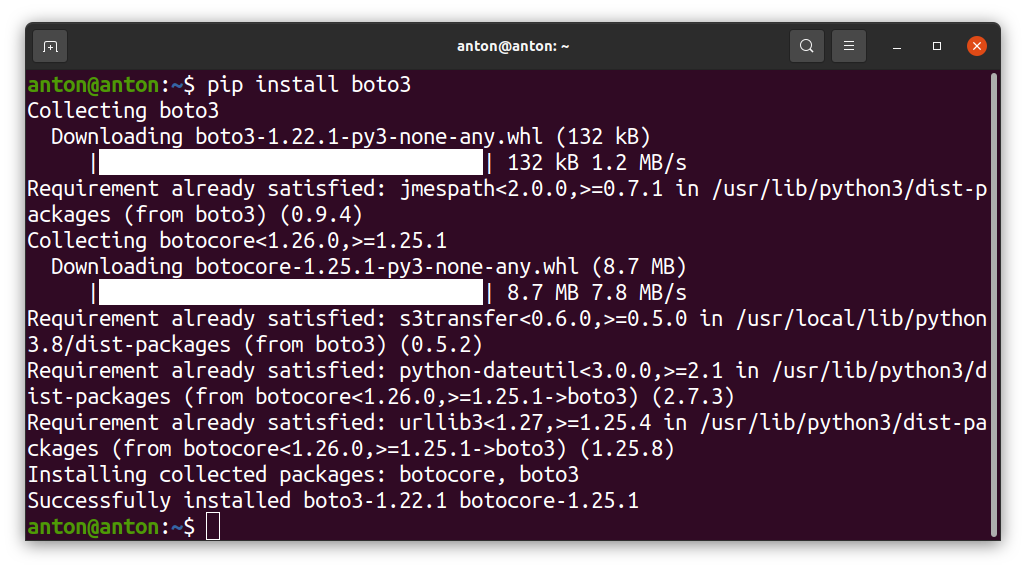
\includegraphics[width=0.93\linewidth]{1/0.1.png}}
    \caption{Завантаження бібліотеки boto3}
    \label{fig:EC2:downloading boto3}
\end{figure}

\begin{figure}[H]
    \begin{minipage}[H]{1\linewidth}
        \center{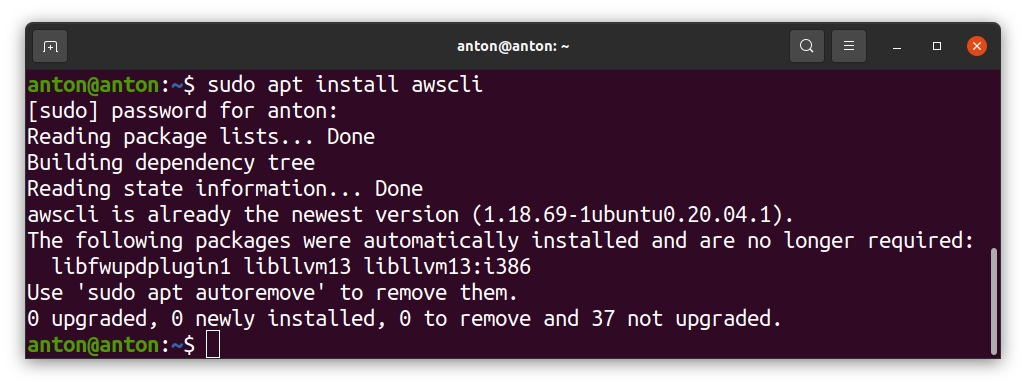
\includegraphics[width=0.93\linewidth]{1/0.2.png}}
    \end{minipage}
    \vfill
    \begin{minipage}[H]{1\linewidth}
        \center{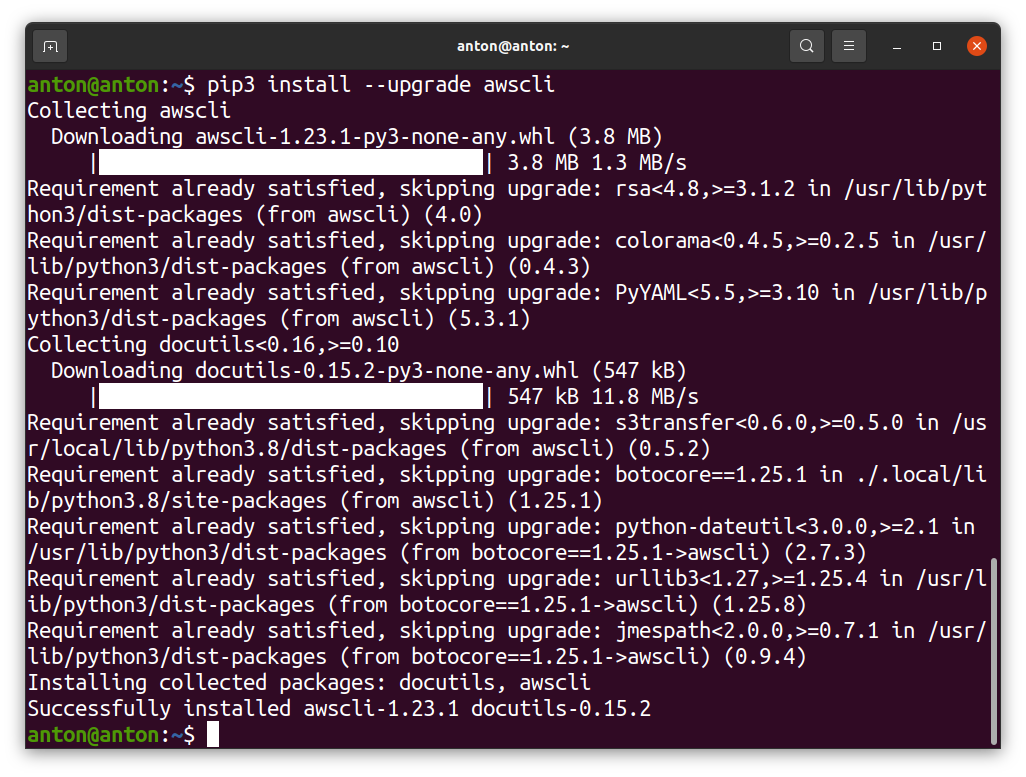
\includegraphics[width=0.93\linewidth]{1/0.3.png}}
        \caption{Встановлення інструментів AWS CLI}
        \label{fig:EC2:downloading awscli}
    \end{minipage}
\end{figure}

\begin{figure}[H]
    \center{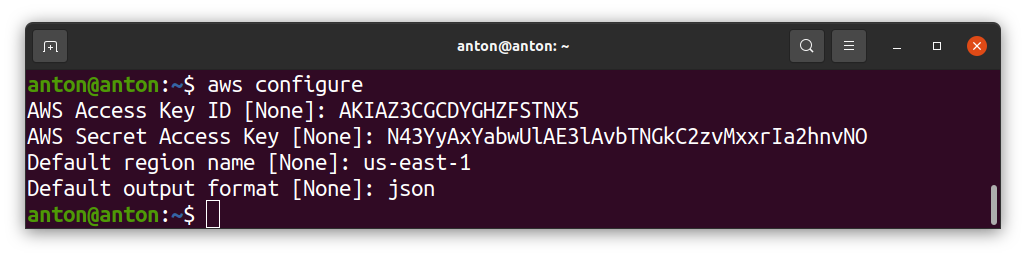
\includegraphics[width=0.93\linewidth]{1/0.4.png}}
    \caption{Підключення до акаунту AWS}
    \label{fig:EC2:connecting to aws}
\end{figure}

\subsubsection*{Створення пари ключів для доступу до EC2-інстансу}

Виконавши усі підготовчі кроки, створюємо файл відповідного розширення (наприклад, \texttt{lab4.py}). Надалі 
будемо поповнювати цей файл кодом й запускатити його в терміналі командою
\[ \texttt{python3 lab4.py} \]

Отже, напишемо функцію створення пари ключів (Лістинг \ref{create a key pair}). Рядком 6 задамо пеараметри інстансу 
та регіону, рядком 7 -- ім'я для ключа, ну і 9 рядком запишемо назву файлу розширення \texttt{.pem}. Фактично, однією 
функцією одразу виконали усі кроки, які ми виконували для відповідного завдання у першій лабораторній роботі. 
Останнім рядком викликаємо функцію \texttt{create\_key\_pair()}. Запустивши файл на виконання, отримуємо бажаний 
результат (Рис.~\ref{fig:EC2:creating key pair}).

\lstinputlisting[firstnumber=1, firstline=1, lastline=13, label = create a key pair, caption = Створення пари ключів]{Code/lab4.py}

\begin{figure}[H]
    \center{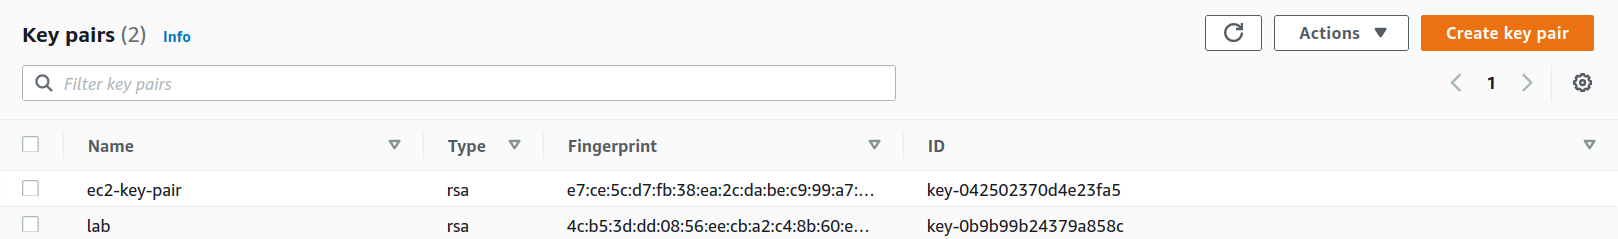
\includegraphics[width=1\linewidth]{1/1.1.png}}
    \caption{Успішно створена пара ключів}
    \label{fig:EC2:creating key pair}
\end{figure}

\subsubsection*{Створення EC2-інстансу}

Наступним кроком створимо власне сам інстанс (Лістинг \ref{create an instance}). Напишемо відповідну функцію 
\texttt{create\_instance()} й вкажемо усі необхідні параметри, серед яких -- ім'я щойно записаного ключа. 
Стосовно параметра <<ImageId>>, то на Рис. \ref{fig:EC2:ami} показано, що його можна знайти на першому кроці 
при стробі створити інстанс через інтерфейс AWS (сам параметр виділено сірим кольором). Рядком 25 забеспечуємо 
вивід <<InstanceId>> після виклику функції.

Запускаємо файл на виконання й переконуємося, що новий інстанс є у переліку усіх інстансів 
(Рис.~\ref{fig:EC2:creating an instance}).

\lstinputlisting[firstnumber=15, firstline=15, lastline=27, label = create an instance, caption = Створення інстансу]{Code/lab4.py}

\begin{figure}[H]
    \center{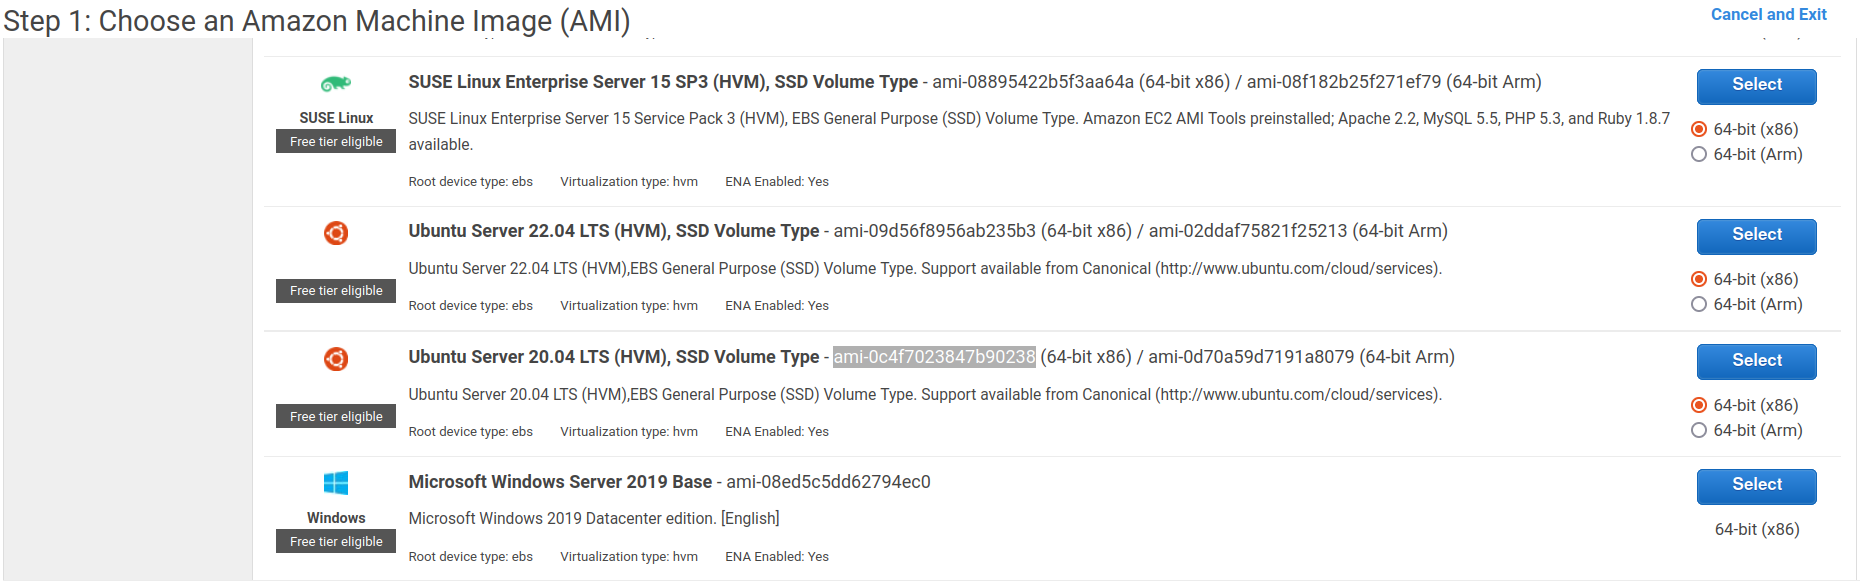
\includegraphics[width=1\linewidth]{1/1.2.png}}
    \caption{Параметр <<ImageId>>}
    \label{fig:EC2:ami}
\end{figure}

\begin{figure}[H]
    \begin{minipage}[H]{1\linewidth}
        \center{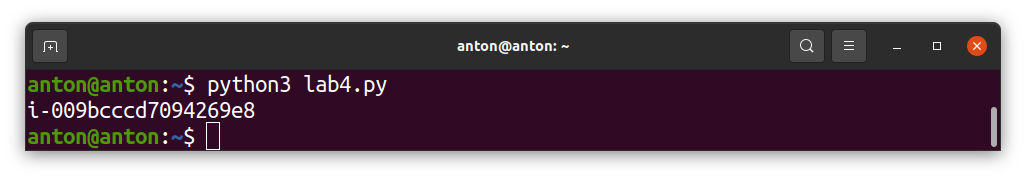
\includegraphics[width=1\linewidth]{1/1.3.png}}
    \end{minipage}
    \vfill
    \begin{minipage}[H]{1\linewidth}
        \center{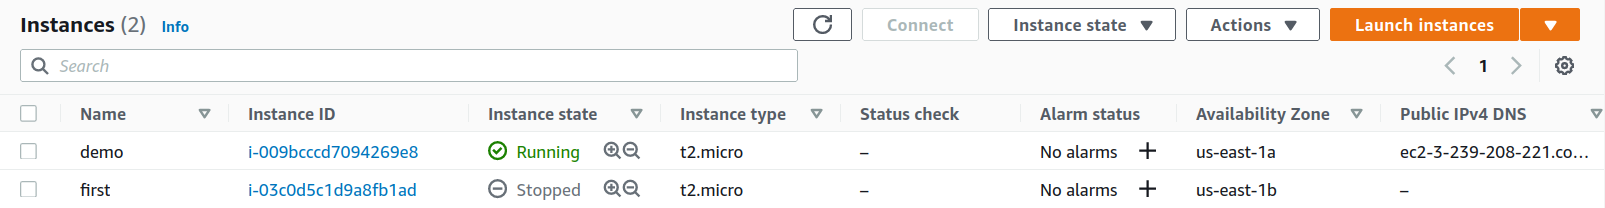
\includegraphics[width=1\linewidth]{1/1.4.png}}
        \caption{Створення інстансу}
        \label{fig:EC2:creating an instance}
    \end{minipage}
\end{figure}

Опісля можемо виконати один додатковий крок -- перевірити, які інстанси зараз запущені на нашому акаунті AWS. 
Сконструюємо доволі громіздку функцію \texttt{get\_running\_instances()}, де у рядках 30-39 фільтром вкажемо 
тип інстансів, які ми хочемо бачити (конкретно 34 рядок -- хочемо виводити саме запущені інстанси). Змінивши 
параметри фільтру, можна вивдити, наприклад, і зупинені інстанси.

А рядками 41-47 для більшої інформативності напишемо код виведення параметрів <<instance\_id>>, <<instance\_type>>, 
<<public\_ip>> та <<private\_ip>>. Результати на Рис.~\ref{fig:EC2:active instances} збігаються із результатами 
на Рис. \ref{fig:EC2:creating an instance} (ба більше, ще й маємо публічні та приватні IP адреси).

\lstinputlisting[firstnumber=29, firstline=29, lastline=49, label = active instances, caption = Моніторинг активних сеансів]{Code/lab4.py}

\begin{figure}[H]
    \center{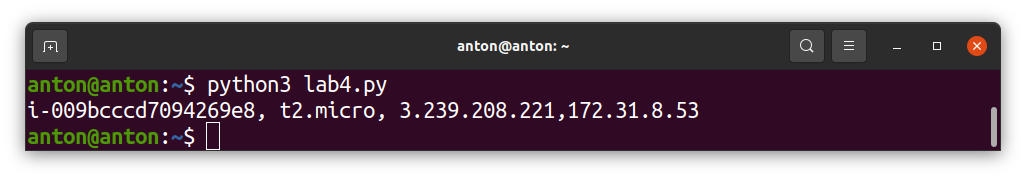
\includegraphics[width=1\linewidth]{1/1.5.png}}
    \caption{Перелік активних сеансів}
    \label{fig:EC2:active instances}
\end{figure}

\subsubsection*{Зупинка й видалення інстансу}

На Лістингу \ref{stop an instance} та \ref{terminate an instance} прописаний код зупинки й видалення інстансу. 
Ключовим параметром є ID інстансу, який ми отримали ще на етапі Рис.~\ref{fig:EC2:creating an instance}. 
Як результат -- відповідні позначки <<Instance state>> для інстансу <<demo>> 
(Рис.~\ref{fig:EC2:stop an instance} та Рис.~\ref{fig:EC2:terminate an instance}).

\lstinputlisting[firstnumber=51, firstline=51, lastline=56, label = stop an instance, caption = Запуника активного інстансу]{Code/lab4.py}

\begin{figure}[H]
    \begin{minipage}[H]{1\linewidth}
        \center{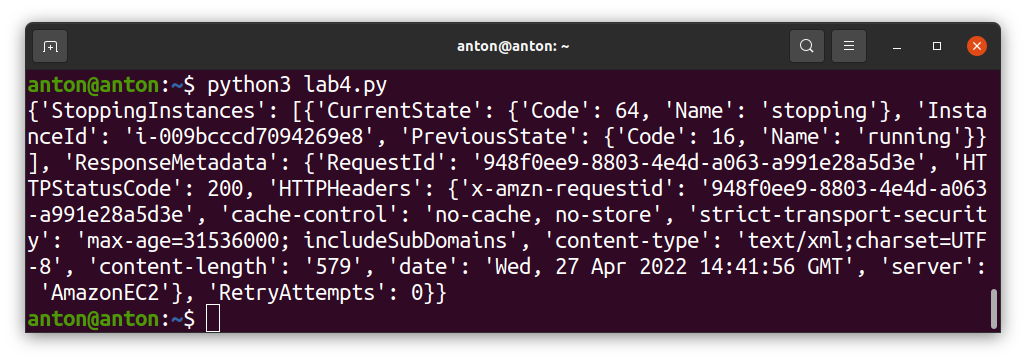
\includegraphics[width=1\linewidth]{1/2.1.png}}
    \end{minipage}
    \vfill
    \begin{minipage}[H]{1\linewidth}
        \center{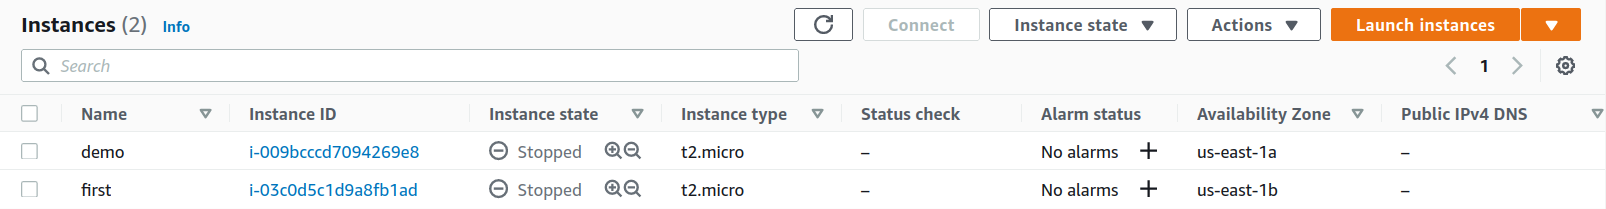
\includegraphics[width=1\linewidth]{1/2.2.png}}
        \caption{Зупинений інстанс}
        \label{fig:EC2:stop an instance}
    \end{minipage}
\end{figure}

\lstinputlisting[firstnumber=58, firstline=58, lastline=63, label = terminate an instance, caption = Видалення зупиненого інстансу]{Code/lab4.py}

\begin{figure}[H]
    \begin{minipage}[H]{1\linewidth}
        \center{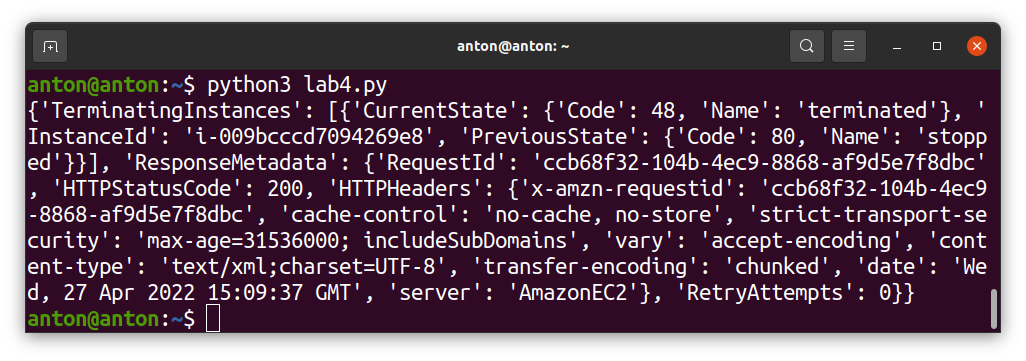
\includegraphics[width=1\linewidth]{1/3.1.png}}
    \end{minipage}
    \vfill
    \begin{minipage}[H]{1\linewidth}
        \center{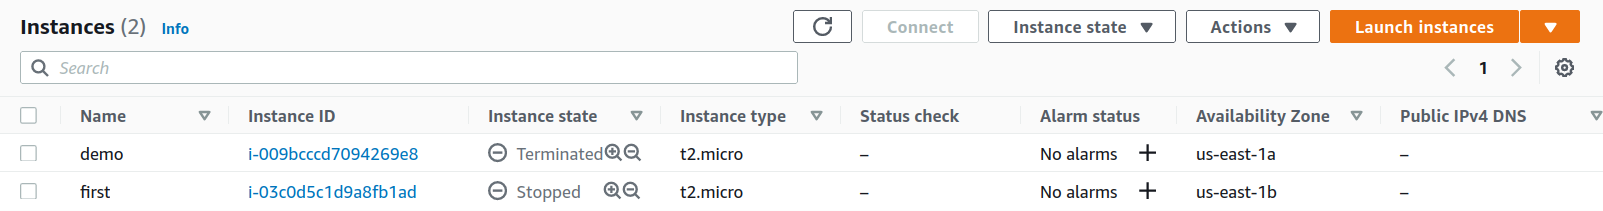
\includegraphics[width=1\linewidth]{1/3.2.png}}
        \caption{Видалений інстанс}
        \label{fig:EC2:terminate an instance}
    \end{minipage}
\end{figure}

\subsection*{2. Автоматизація роботи з сховищем S3}

\subsubsection*{Cтворення бакета S3}

Для створення бакету реалізуємо функцію \texttt{create\_bucket()}, якій передамо параметри імені нового бакету 
та регіону. Аналогічно до об'єкту \texttt{ec2\_client} у попередньому розділі, на цей раз всі необхідні методи 
для керування бакетом можемо отримати через об'єкт \texttt{s3\_client}.

\lstinputlisting[firstnumber=65, firstline=65, lastline=76, label = create S3, caption = Створення бакету S3]{Code/lab4.py}

\begin{figure}[H]
    \begin{minipage}[H]{1\linewidth}
        \center{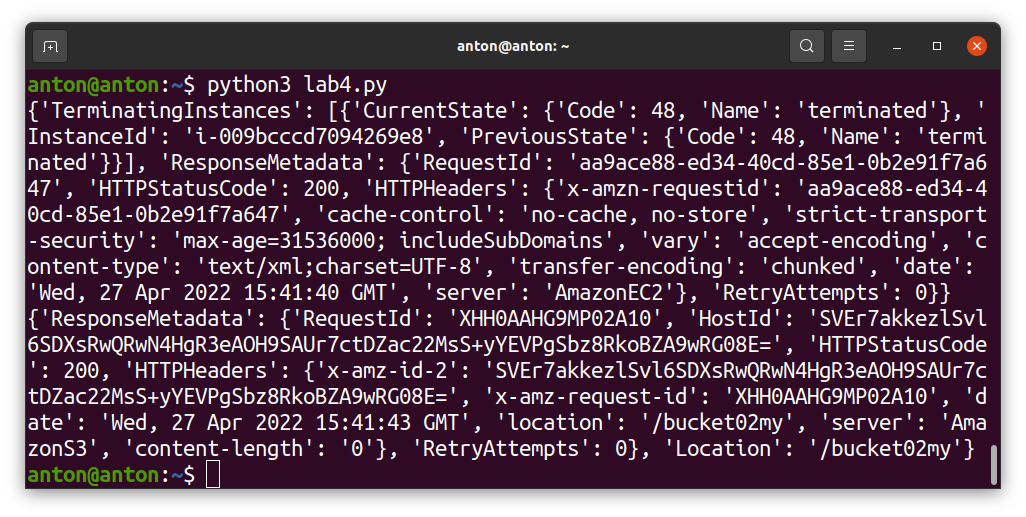
\includegraphics[width=1\linewidth]{2/1.1.png}}
    \end{minipage}
    \vfill
    \begin{minipage}[H]{1\linewidth}
        \center{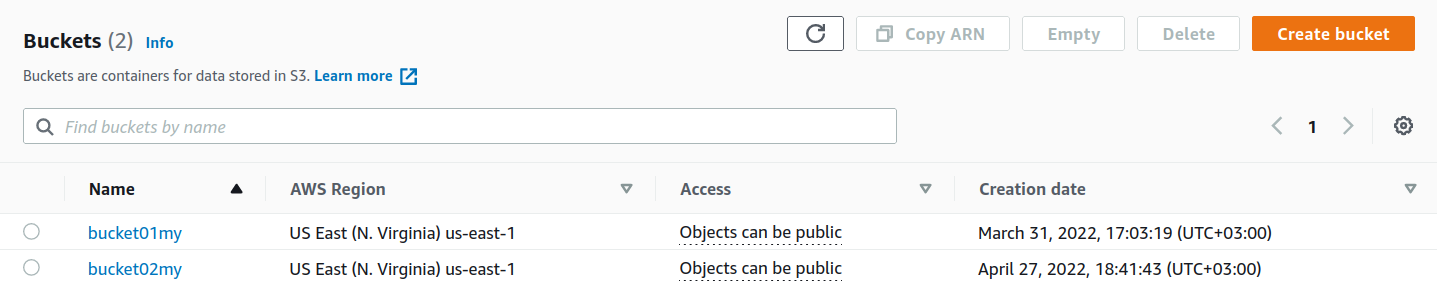
\includegraphics[width=1\linewidth]{2/1.2.png}}
        \caption{Створений бакет}
        \label{fig:S3:create a bucket}
    \end{minipage}
\end{figure}

У Лістингу \ref{create S3} конструкція \texttt{try: except} аналогічна конструкції \texttt{try: catch} в 
інших мовах програмування й покликана <<зловити>> виняткові ситуації помилок. Наприклад, у рядку 71 <<ловимо>> 
помилку неприйнятної довжини для імені, а у рядку 73 -- проблему неунікального імені бакету. 

Між іншим, назва помилки \texttt{botocore.exceptions.ClientError} була витягнута безпосередньо з консолі 
терміналу. Отже, після уникнення помилок хибних імен бакету, маємо остаточний результат, який показано на Рис. 
\ref{fig:S3:create a bucket}.

Аналогічно до етапу створення інстансу, останнім кроком цього пункту можемо написати код моніторингу активних 
бакетів (Лістинг \ref{active buckets}). Як результат -- маємо бажаний перелік (Рис. \ref{fig:S3:active buckets}).

\lstinputlisting[firstnumber=78, firstline=78, lastline=86, label = active buckets, caption = Активні бакети]{Code/lab4.py}

\begin{figure}[H]
    \center{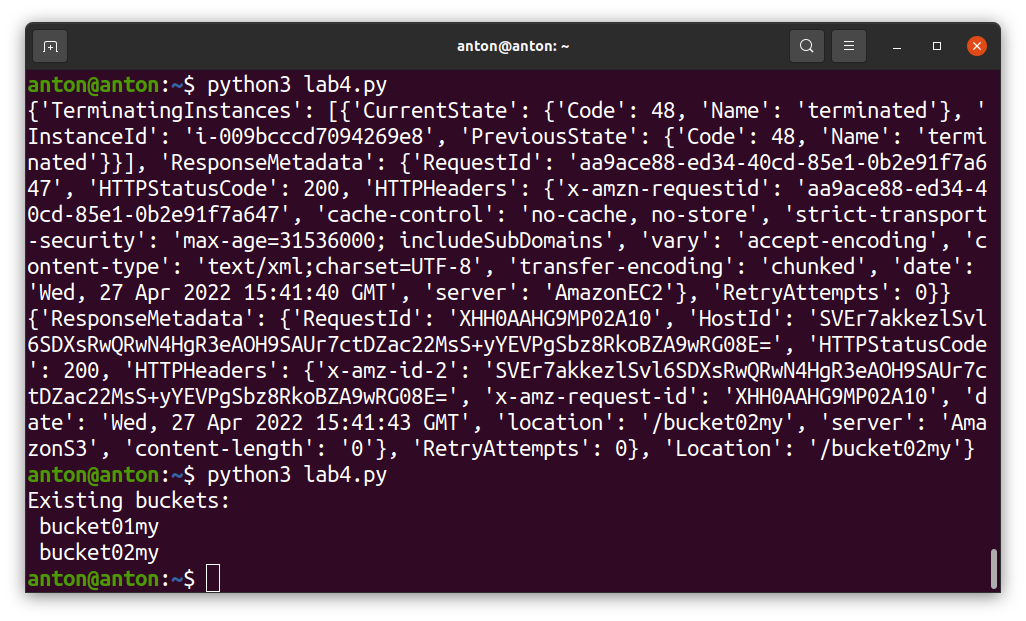
\includegraphics[trim=0cm 0cm 0cm 16.25cm, clip, width=1\linewidth]{2/1.3.png}}
    \caption{Перелік існуючих бакетів}
    \label{fig:S3:active buckets}
\end{figure}

\subsubsection*{Завантаження й читання даних}

Завантажимо на новостворений бакет файл з курсом валют, який ми використовували у Лабораторній роботі 
\textnumero2. До речі, необхідний нам файл \texttt{request.csv} досі лежить на попередньому бакеті 
(Рис. \ref{fig:S3:active buckets}), створеному у тій же другій лабораторній. Тож зайшовши на бакет 
\texttt{bucket01my}, завантажую на локальне сховище шукані дані. Отже, передаю у функцію \texttt{upload()} 
назву оригінального файлу та ім'я, яке він матиме на бакеті \texttt{bucket02my}. 

\lstinputlisting[firstnumber=88, firstline=88, lastline=93, label = download file on S3, caption = Завантаження файлу на бакет]{Code/lab4.py}

\begin{figure}[H]
    \center{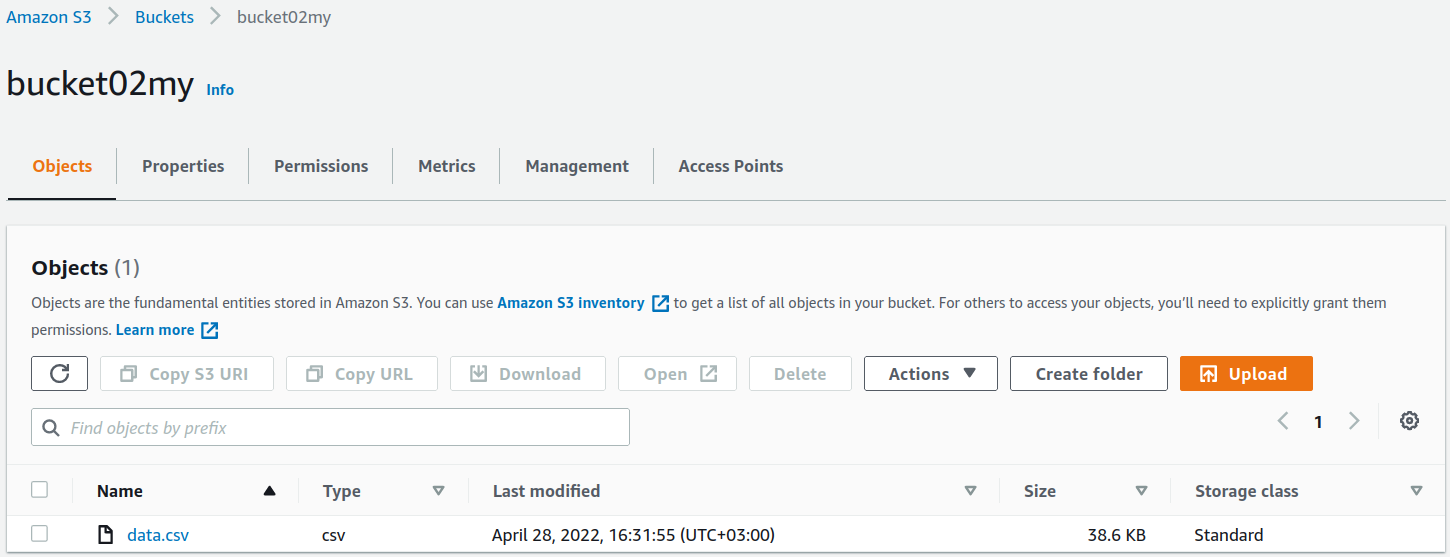
\includegraphics[width=1\linewidth]{2/2.2.png}}
    \caption{Вивантажений на бакет файл}
    \label{fig:S3:upload a file}
\end{figure}

Як бачимо, завантаження пройшло успішно (Рис. \ref{fig:S3:upload a file}). Тепер зчитаємо із цього файлу інформацію 
про перші рядки таблиці. Для візуалізації даних окремо встановимо відповідну бібліотеку \texttt{pandas} командою
\[ \texttt{pip3 install pandas} \]

Наразі приймемося до написання функції \texttt{printing\_data\_from\_s3()}. Основним є 101 рядок 
(Лістинг \ref{read file from S3}). А рядками 105 та 107 <<ловимо>> й інформуємо користувача про помилки 
звернення до бакету чи файлу з неіснуючим іменем. 

\lstinputlisting[firstnumber=95, firstline=106, lastline=121, label = read file from S3, caption = Зчитування даних з бакету]{Code/lab4.py}

У рядках 106 та 108 текст помилок не виділений відповідним кольором виключно через технічні складнощі середи 
\LaTeX{} у відображенні в блоках коду символів нелатинського алфавіту. Результати помилкових запитів до бакету 
й власне успішне читання даних зображені на Рис. \ref{fig:S3:read a file}.

\begin{figure}[H]
    \center{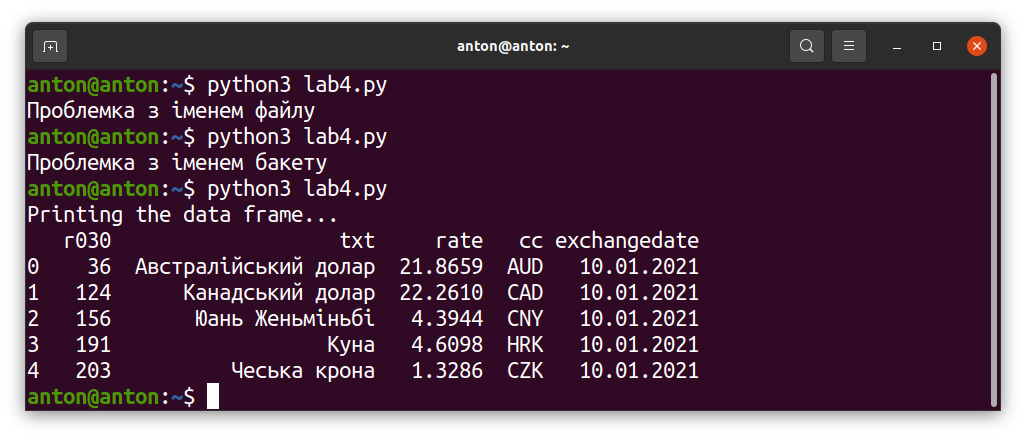
\includegraphics[width=1\linewidth]{2/2.5.png}}
    \caption{Читання з файлу}
    \label{fig:S3:read a file}
\end{figure}

\subsubsection*{Видалення бакету S3}

Ну і наостанок видалимо бакет з іменем \texttt{bucket02my}. Щоправда мушу зазначити, що метод 
\texttt{s3\_client.delete\_bucket()} видаляє лише порожні бакети, тому спершу слід видалити усі зайві файли 
(як це зроблено для файлу \texttt{data.csv} у рядку 116 Лістингу \ref{delete bucket}). Тож викликавши файл 
на виконання, переконаємося, що бакет справді видалений, за допомогою раніше написаної функції 
\texttt{printing\_buckets()}. Результати успішного виконання -- на Рис. \ref{fig:S3:delete a bucket}.

\lstinputlisting[firstnumber=112, firstline=95, lastline=104, label = delete bucket, caption = Видалення бакету]{Code/lab4.py}

\begin{figure}[H]
    \center{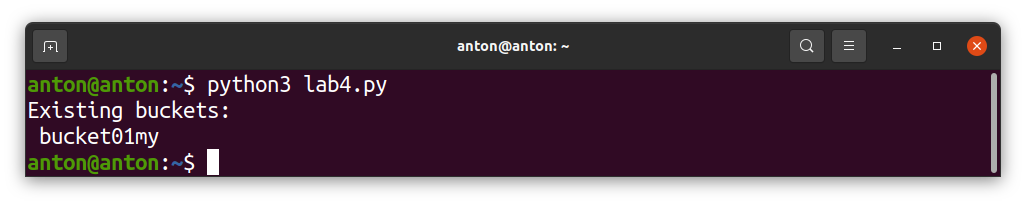
\includegraphics[width=1\linewidth]{2/3.2.png}}
    \caption{Перевірка видалення бакету}
    \label{fig:S3:delete a bucket}
\end{figure}

\subsection*{3. Робота з git-репозиторієм}

Наведу ще раз умову завдання цього етапу: для результатів Лабораторної роботи \textnumero2 розробити 
bash-скрипт, який склонує код з попередньо створеного git-репозиторію та встановить потрібні заленості 
\texttt{pip}. Тож з постановки завдання можна виокремити декілька підкроків:
\begin{itemize}
    \item Підготувати на локальному сховищі такі два файли:
    \begin{align*}
        &\texttt{lab2.py} && \text{код Лабораторної роботи \textnumero2} \\
        &\texttt{requirements.txt} && \text{перелік бібліотек та пакетів \texttt{pip}}
    \end{align*}
    \item Відкрити git-репозиторій та зберегти зазначені вище файли на ньому;
    \item На локальному сховищі написати необхідний bash-скрипт;
    \item Перекинути bash-скрипт на новостворений інстанст й запустити його.
\end{itemize}

Як результат: завдяки встановленню необхідних бібліотек та пакетів з файлу \texttt{requirements.txt} код 
\texttt{lab2.py} з Лабораторної роботи \textnumero2 має запуститися й успішно виконатися на новому інстансі. 

\subsubsection*{Крок 1: підготовка програмних файлів}

Перш за все я віднайшов файл з кодом \texttt{lab2.py}, суть якого полягала у візуалізації даних про курс валют 
протягом 2021 року. Маючи інструмент \texttt{pip} встановленим, настуаним кроком командою 
\[ \texttt{pip3 freeze > requirements.txt} \]
я формую текстовий файл із назвами відповідних пакетів та бібліотек. На Рис.~\ref{fig:git:prepare files} 
показано процес створення відповідного файлу та перевірки його наповнення (демонструється лише початок файлу).

\subsubsection*{Крок 2: відкриття git-репозиторію}

Створивши акаунт на \url{https://github.com} (або маючи вже створений), відкриваємо новий репозиторій. Усі 
подальші кроки можна виконувати як інструментами \texttt{git} через термінальний рядок, так і за допомогою 
інтерфейсу самого сайту. Я виконуватиму роботу через другий варіант: тож обираємо <<uploading an existing file>> 
та завантажуємо підготовані на Кроці 1 файли. Результати й процес виконання зображені на Рис~\ref{fig:git}.

Назагал, нам ще зустрінеться робота з утилітою \texttt{git}, тож для попереднього тестування й 
ознайомлення цей інструмент можна завантажити на своє локальне сховище завдяки команді 
\texttt{sudo apt install git}.

\begin{figure}[H]
    \center{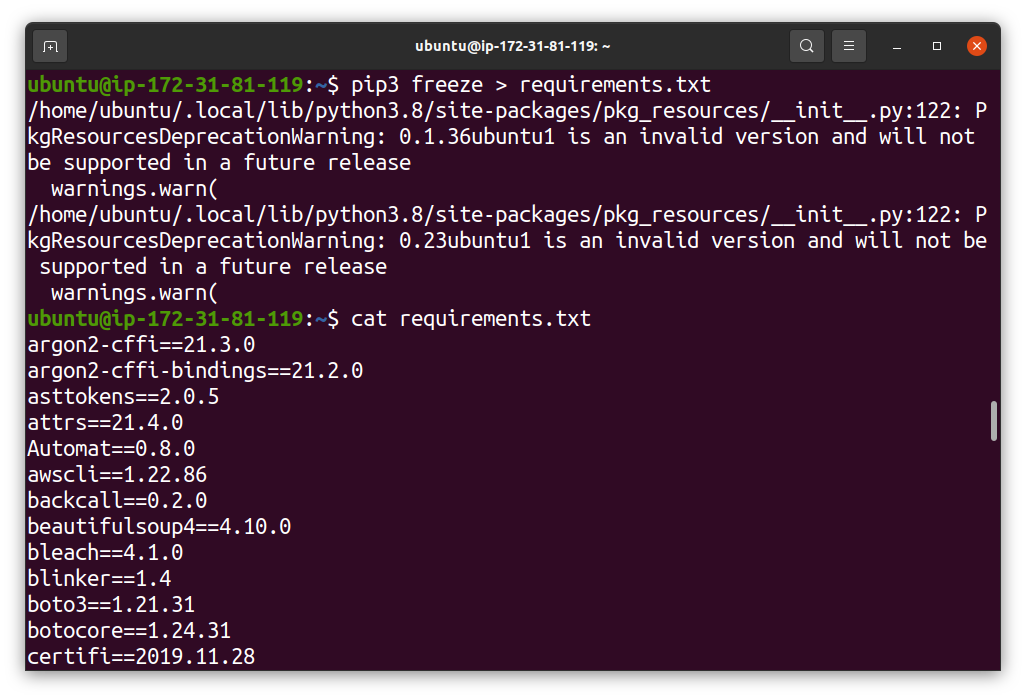
\includegraphics[width=1\linewidth]{3/1.png}}
    \caption{Підготовка необхідних файлів}
    \label{fig:git:prepare files}
\end{figure}

\begin{figure}[H]
    \begin{minipage}[H]{1\linewidth}
        \center{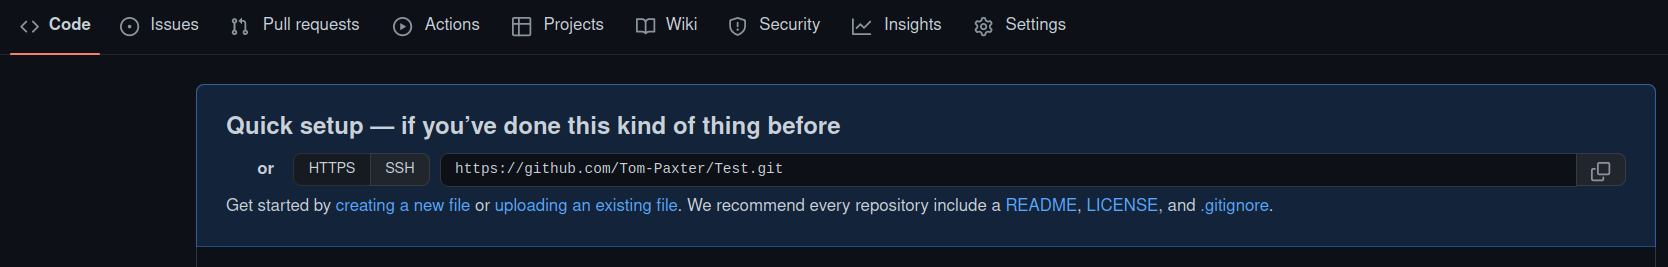
\includegraphics[width=1\linewidth]{3/2.1.png}}
    \end{minipage}
    \vfill
    \begin{minipage}[H]{1\linewidth}
        \vspace{0.2cm}\center{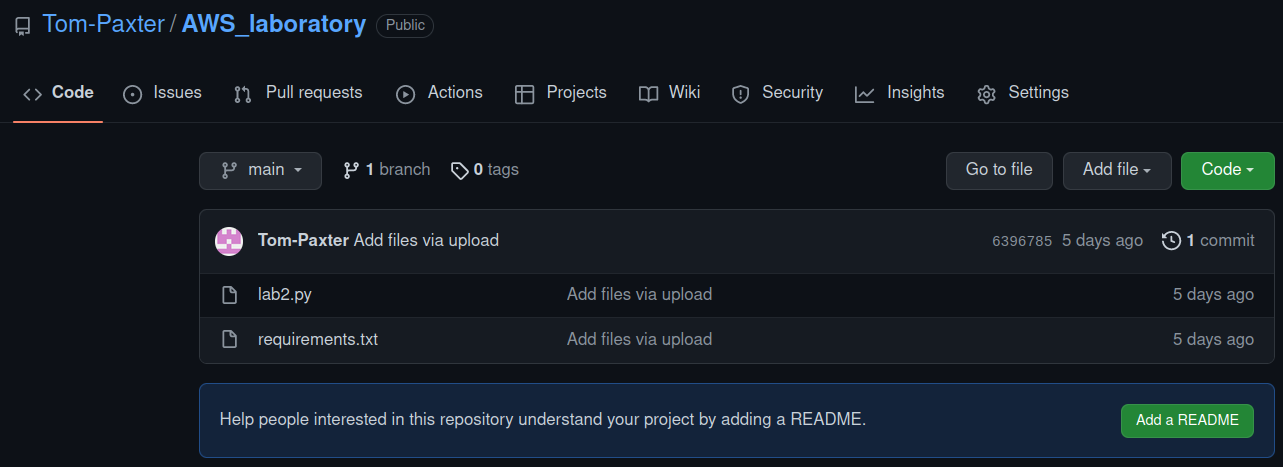
\includegraphics[width=1\linewidth]{3/2.2.png}}
        \caption{Завантаження файлів на репозиторій}
        \label{fig:git}
    \end{minipage}
\end{figure}

\subsubsection*{Крок 3: створення bash-скрипта}

Bash-скрипт являє собою файл з набором термінальних команд. Тож створимо файл \texttt{commands.sh} приблизно такого змісту:

\begin{lstlisting}[language=bash, stringstyle=\small\ttfamily, emphstyle={[1]\small\ttfamily}]
    #!/bin/bash

    sudo apt update
    sudo apt install git
    git clone https://github.com/Tom-Paxter/AWS_laboratory.git
    sudo apt install python3-pip
    while read requirement; do pip3 install $requirement; done < AWS_laboratory/requirements.txt
    
\end{lstlisting}

Завдання скрипта полягає у тому, щоб при його запуску на новому інстансі були встановлені усі необхідні 
інструменти для виконання програмного файлу \texttt{lab2.txt}. Кожен рядок коду виконує таку функцію:
\begin{align*}
    &\circ \texttt{sudo apt update} && \parbox[t]{10cm}{оновлення дерева пакетів для подальшого 
    завантаження наступних інструментів;} \\
    &\circ \texttt{sudo apt install git} && \parbox[t]{10cm}{встановлення термінальної утиліти \texttt{git};} \\
    &\circ \texttt{git clone} && \parbox[t]{10cm}{копіювання із репозиторію (url репозиторію)  файлів 
    \texttt{lab2.py} та \texttt{requirements.txt};} \\
    &\circ \texttt{sudo apt install python3-pip} && \parbox[t]{10cm}{завантаження менеджера \texttt{pip};} \\
    &\circ \texttt{while read requirement;} && \parbox[t]{10cm}{завантаження необхідних пакетів \texttt{pip} 
    з вказаного файлу \texttt{requirements.txt}}
\end{align*}

Замість команди в рядку 7 спершу була використана більш зрозуміла на вигляд команда 
\[ \texttt{pip3 install -r AWS\_laboratory/requirements.txt} \]
Проте її виконання призводило до певних помилок, тому її довелося модифікувати (детальніше про цю проблему 
в заключному розділі).

\subsubsection*{Крок 4: перевірка результатів завдання}

Отже, наостанок залишилося створити новий інстанс, пернекинути на нього файл bash-скрипта та перевірити виконання 
завдання. Перш за все створюємо новий інстанс (Рис. \ref{fig:git:create new instance}), потім перекидаємо файл 
(Рис. \ref{fig:git:copy file}) й перевіряємо його наявність на новому інстансі (Рис. \ref{fig:git:check file}).

\begin{figure}[H]
    \center{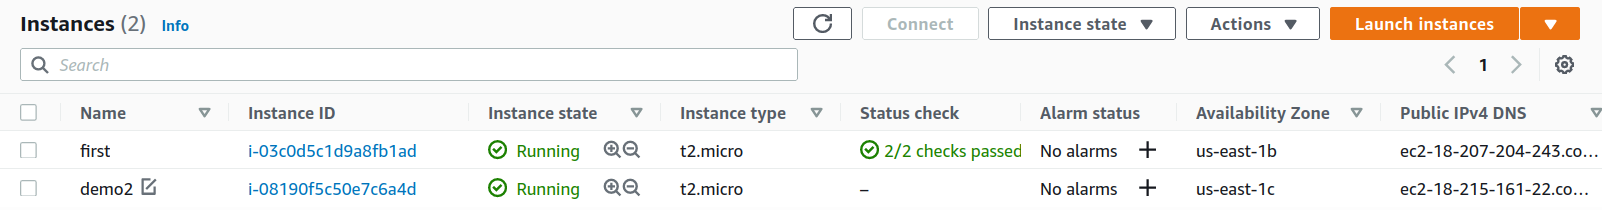
\includegraphics[width=1\linewidth]{3/4.1.png}}
    \caption{Новий інстанс <<demo2>>}
    \label{fig:git:create new instance}
\end{figure}

\begin{figure}[H]
    \center{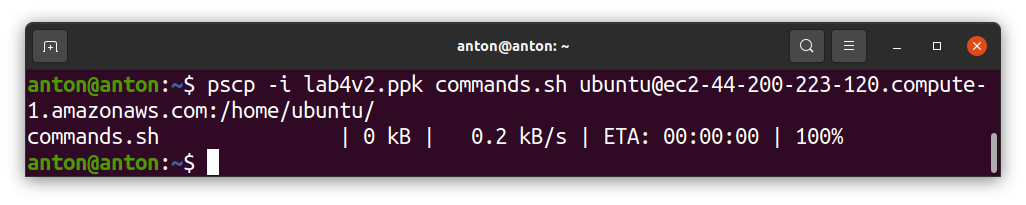
\includegraphics[width=1\linewidth]{3/4.2.png}}
    \caption{Копіювання файлу на новий істанс}
    \label{fig:git:copy file}
\end{figure}

\begin{figure}[H]
    \center{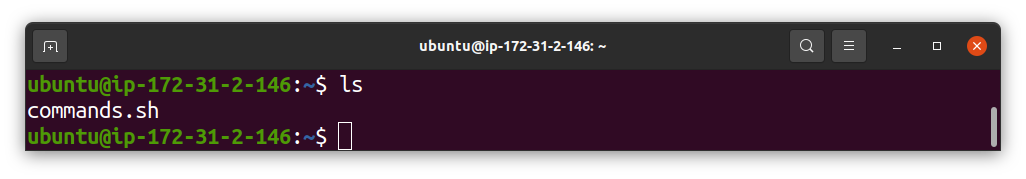
\includegraphics[width=1\linewidth]{3/4.3.png}}
    \caption{Перевірка успішного копіювання}
    \label{fig:git:check file}
\end{figure}

Усі підготовчі кроки виконано, тож нарешті підключаємося до інстансу й запускамо bash-скрипт простою 
термінальною командою
\[ \texttt{bash commands.sh} \]

Якщо все виконано правильно, то на новий порожній інстанст почнеться завантаження необхідного програмного 
забеспечення (показано на Рис~\ref{fig:git:install pip} та Рис. \ref{fig:git:install git}).

\begin{figure}[H]
    \center{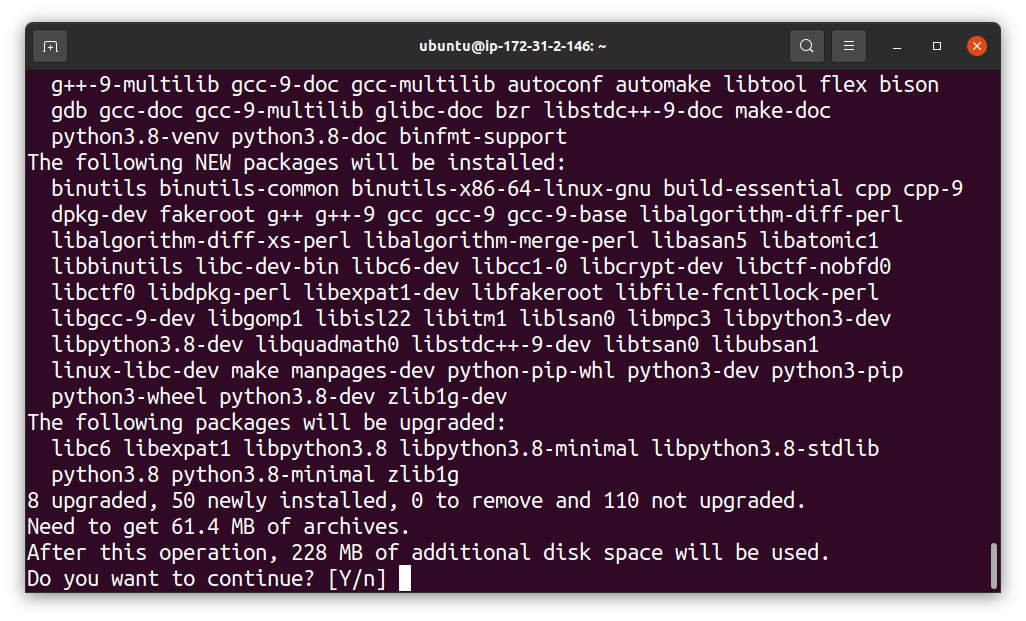
\includegraphics[width=1\linewidth]{3/4.4.png}}
    \caption{Завантаження менеджера \texttt{pip}}
    \label{fig:git:install pip}
\end{figure}

\begin{figure}[H]
    \center{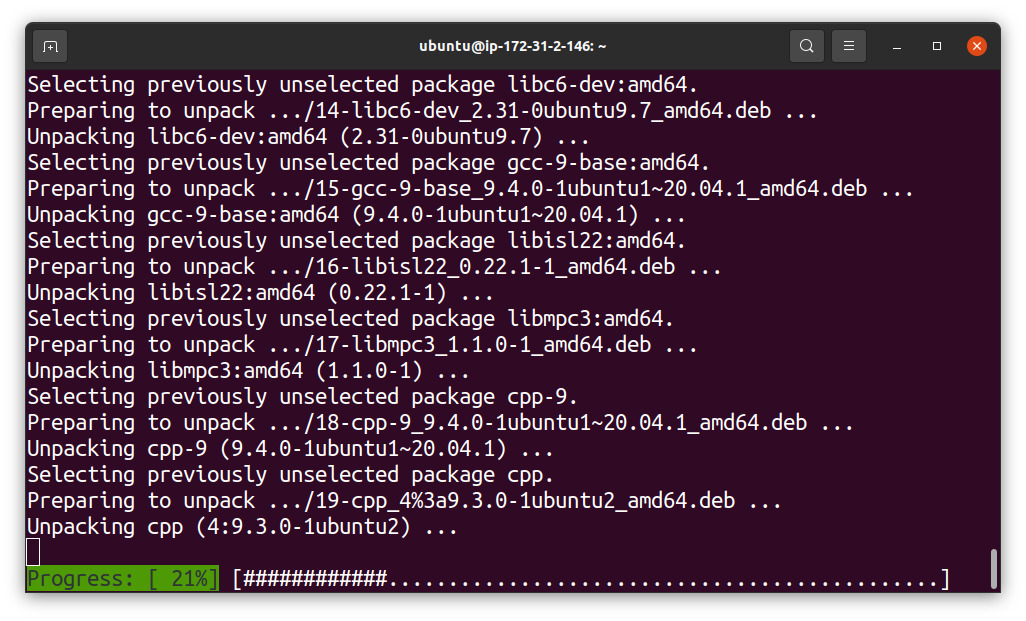
\includegraphics[width=1\linewidth]{3/4.5.png}}
    \caption{Процес завантаження необхідного ПЗ}
    \label{fig:git:install git}
\end{figure}

Остаточно переконуємося в наявності бажаних файлів (Рис \ref{fig:git:check files on instance}) й запускаємо 
на виконання \texttt{lab2.py}. Як результат -- отримуємо поповнення в дереві файлів: щонайменше малюнок курсу 
валют \texttt{exchange\_rate.png} (Рис. \ref{fig:git:final check}).

\begin{figure}[H]
    \center{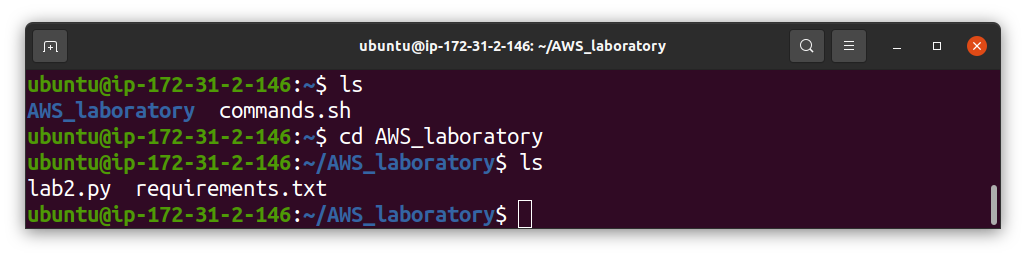
\includegraphics[width=1\linewidth]{3/4.6.png}}
    \caption{Перевірка наявності файлів}
    \label{fig:git:check files on instance}
\end{figure}

\begin{figure}[H]
    \center{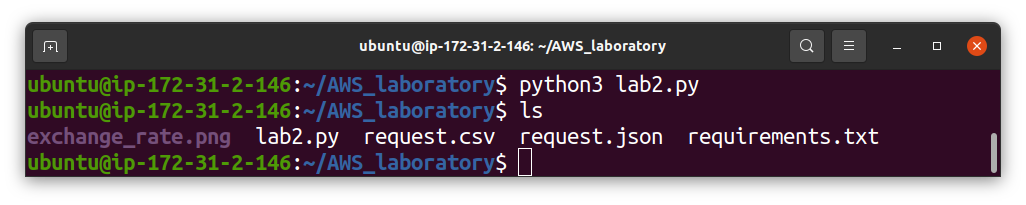
\includegraphics[width=1\linewidth]{3/4.7.png}}
    \caption{Фінальна перевірка завданння}
    \label{fig:git:final check}
\end{figure}

\subsection*{4. Перелік проблем протягом виконання роботи}

\begin{enumerate}
    \item Аналогічно до проблеми Лабораторної роботи \textnumero2 зіткнувся з питанням 
    некоректного завантаженням інструментів AWS CLI. Вдалося вирішити непорозуміння завдяки додатковому
    оновленню утиліт командою
    \[ \texttt{pip3 install --upgrade awscli} \]
    \item Назагал, робота з git-репозиторієм є для мене новим досвідом. Створений акаунт я вже мав, проте 
    реальної потреби зберігати на ньому певний код не виникало. Через відсутність практичних навичок були 
    певні труднощі в опануванні термінального менеджера \texttt{git} -- не вдалося створити репозиторії й 
    перекинути туди бажані файли. Тому вирішив піти іншим шляхом (як не прикро, але шляхом новачка) -- 
    взаємодія з інтерфейсом сайту \url{https://github.com}.
    \item При створенні bash-скрипта, як це вже зазначалося раніше, виникли проблеми із способом завантаження 
    пакетів \texttt{pip} через команду \[ \texttt{pip3 install -r AWS\_laboratory/requirements.txt} \]

    Зіткнувся з аналогічною проблемою, яка зазначена 
    \href{https://stackoverflow.com/questions/44031496/how-to-continue-with-the-instalation-of-the-following-packages-after-an-error}{тут}. 
    У цій же статті віднайшов коректний спосіб оминати завантаження <<проблемних>> для терміналу бібліотек.
\end{enumerate}

\end{document}